\chapter{Analyse}

\section{Einordnung des Kreditorenworkflows}
Um die Intention der Neukonzeption verstehen und sie angemessen durchführen zu können, ist es zunächst wichtig, den Workflow der Kreditorenbuchhaltung im Unternehmen einordnen zu können, um Verständnis für die Anforderungen zu bekommen. 
Dieser Umstand ist analog zu den Anforderungen der ISO 9000 Reihe zu sehen, das zur Qualitätssicherung in Prozessen ein Verständnis von deren Abhängigkeiten und Wechselwirkungen vorgibt. \\
Die Einordnung in das Prozessportfolio kann z.B. auf Grundlage von Six Sigma erfolgen.
Dazu werden die strategische Relevanz (bzw. Bedeutung für den Geschäftserfolg) und der Verbesserungsbedarf gegenübergestellt. 
Diese Gegenüberstellung erfolgt qualitativ und auf Basis der Einschätzung von Stakeholdern.
Je  Dimension sind mehrere Kriterien (Strategische Bedeutung: Marktrelevanz, Geschäftskritikalität, Marktfähigkeit; Verbesserungsfähigkeit: Technologische Unterstützung, Fehleranfälligkeit, Performance) zu bewerten. 
Das Mittel aller Einschätzungen ergibt die Positionierung im Portfolio-Diagramm.

\begin{figure}[!htb]
\centering
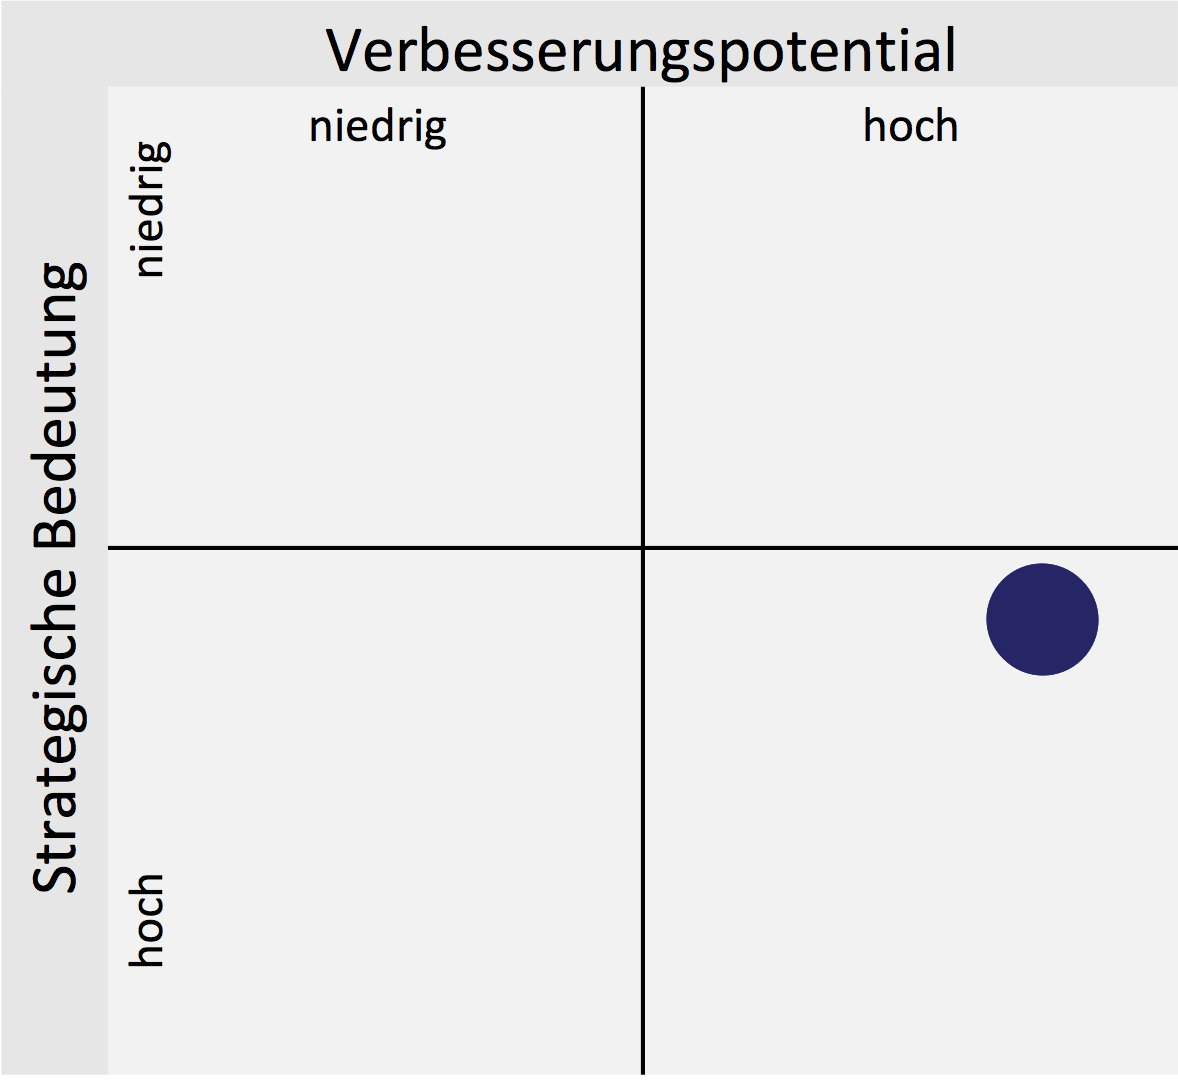
\includegraphics[height=60mm]{images/portfolio}
\caption{Portfolioeinordnung des Kreditorenworkflows}
\label{Portfolioeinordnung des Kreditorenworkflows}
\end{figure}
\footnotetext{Quelle: Autor}

Es ergibt sich ein hohes Verbesserungspotential, dessen Erläuterung Teil dieses Kapitels ist.
Die ebenfalls hohe strategische Relevanz resultiert aus zwei Rahmenbedingungen. 
Zum einen ist die Rechnungslegung gegenüber dem Gesetzgeber verpflichtend und ist daher für den Geschäftsbetrieb unerlässlich. Dieser Umstand alleine, reicht allerdings nicht aus. 
Entscheidend ist, dass die Kreditorenbuchhaltung auch als Service von der \firma angeboten wird.
Das bedeutet konkret, dass Firmen (insbesondere Beteiligungsfirmen, also Bestandteile der GLC Group) die Kreditorenbuchhaltung an die \firma outsourcen können. 
Dementsprechend wird in dem Prozess auch Service gegenüber Kunden generiert.\\
Ordnet man nun diesen Prozess in eine Prozesslandkarte, wie im Rahmen von ISO 9000 beispielsweise üblich, ein, zeigt sich, dass der Prozess nicht ausschließlich, wie bei Inhalten der Finanzbuchhaltung ansonsten üblich, als Unterstützungsprozess einzustufen ist.


\begin{figure}[!htb]
\centering
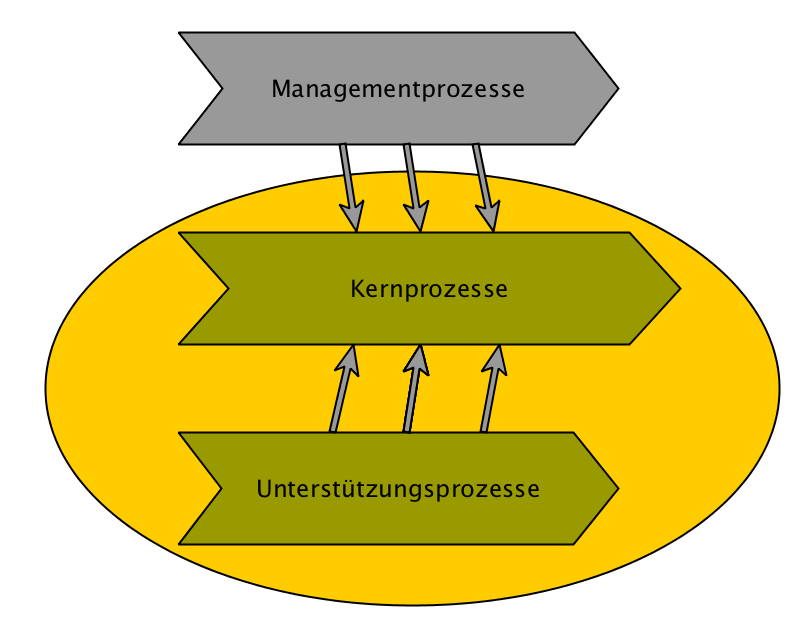
\includegraphics[height=60mm]{images/prozesslandkarte}
\caption{Portfolioeinordnung des Kreditorenworkflows}
\label{Portfolioeinordnung des Kreditorenworkflows}
\end{figure}
\footnotetext{Quelle: Autor}


Vielmehr zeigt sich, dass, je nach Prozessinstanz, die Einordnung zwischen Kernprozess (bzw. Leistungsprozess) und Unterstützungsprozess (bzw. Supportprozess) pendelt. 
Mehrheitlich betreffen die Prozessinstanzen interne Rechnungen, welche als Supportprozess eingeordnet werden. 
Hinsichtlich Kundenrechnungen, welche eher Leistungsprozessinstanzen darstellen, ergeben sich jedoch teilweise differierende Anforderungen an den Prozess.
Dieser Umstand wird im weiteren Verlauf berücksichtigt.


\section{Ist-Aufnahme}
Der Prozess wird in zwei sequentiellen Stufen betrachtet. 
Im ersten Teil geht die Rechnung  ein und wird freigegeben.
Im zweiten Teil wird die Rechnung gebucht und der Zahllauf vorbereitet.
\subsection{Kreditorenworkflow Teil 1: Rechnungsfreigabe}
Der erste Teil beginnt streng genommen mit der Kostenverursachung, auf die eine Kreditorenrechnung folgt. 
Da die Kostenverursachung allerdings für den Workflow nicht weiter relevant ist, wird der Rechnungseingang als Ausgangspunkt des Prozesses und Auslöser einer Prozessinstanz betrachtet. 
\subsubsection{Prozessablauf}
Die eingehende Kreditorenrechnung wird innerhalb des Unternehmens an einen bestimmten Mitarbeiter der Finanzbuchhaltung gegeben.
Für die nachfolgenden Schritte gibt es zwei mögliche Szenarien.

\paragraph{Fall 1: Kostenverursacher in Niederlassung}
~\\ 
In diesem Szenario befindet sich der Kostenverursacher nicht in der Unternehmenszentrale, also in räumlicher Distanz zur Finanzbuchhaltung.\\
Der Mitarbeiter scannt die Rechnung ein, um das Original digital zu konservieren, was den ersten Schritt der Versionierung darstellt. $\rightarrow$
Danach muss die Rechnung zur sachlichen Freigabe an den Kostenverursacher gegeben werden. 
Wird die Rechnung sachlich nicht freigegegeben, endet die Prozessinstanz.
Nachfolgend müssen vom Mitarbeiter der Finanzbuchhaltung die Gründe dafür eruiert und ggf. eine korrekte Rechnung nachgefordert werden.$\rightarrow$
Wird die Rechnung sachlich freigegeben, druckt der freigebende Mitarbeiter dazu die Rechnung aus, unterschreibt und scannt wieder.
Das Resultat sendet er dem Mitarbeiter der Finanzbuchhaltung.
Dieser druckt wiederum das Resultat aus.
Danach muss die fachliche Freigabe erfolgen.
Dazu verbringt der Mitarbeiter die Original-Rechnung und den Ausdruck mit der sachlichen Freizeichnung an den verantwortlichen Bereichsleiter.
Dieser lehnt ggf. die Rechnung ab, dazu wird wie im Fall der sachlichen Freigabe verfahren.
Im Regelfall gibt er mit seiner Unterschrift die Rechnung fachlich frei.
Ggf. erfolgt ein Vermerk, dass die Rechnung an einen Kunden weiterzuberechnen ist. 
Nachdem die fachliche Freigabe erfolgt ist, wird die finale Version eingescannt.\\
Damit liegen alle Freigaben vor und der Mitarbeiter ist zur Buchung berechtigt.

\paragraph{Fall 2: Kostenverursacher in Unternehmenszentrale}
~\\
In diesem Szenario befindet sich der Kostenverursacher in der Unternehmenszentrale, also in für die Mitarbeiter der Finanzbuchhaltung erreichbarer Nähe.
Zunächst muss ebenso die sachliche Freigabe erfolgen.
Dazu verbringt der Mitarbeiter der Finanzbuchhaltung die Original-Rechnung an den Kostenverursacher.
Für eine nicht erfolgte Freigabe wird wie in Fall 1 verfahren.
Bei erfolgter sachlicher Freigabe hat ebenso als nächtes die fachliche Freigabe zu erfolgen.
Wie in Fall 1 wird dazu die Original-Rechnung, diesmal allerdings mit sachlicher Freigabe an den Bereichsverantwortlichen verbracht.
Auch an dieser Stelle wird wie in Fall 1 für Freigabe oder Nicht-Freigabe verfahren.
Ggf. erfolgt auch hier ein Vermerk, der die Weiterberechnung anweist.
Im Regelfall gibt er mit seiner Unterschrift die Rechnung fachlich frei.
Abschließend wird die vollständig freigezeichnete Version eingescannt.
Damit liegen alle Freigaben vor und der Mitarbeiter ist zur Buchung berechtigt.

\subsubsection{Prozessmodellierung}
Der Prozess lässt sich soweit modellieren. 
Zu beachten sind dabei zwei Prozessschnittstellen. 
Eine davon ist die zur Debitorenbuchhaltung, die bei einem Weiterberechnungsvermerk greift. 
Diese wird modelliert, ist allerdings inhaltlich in diesem Rahmen nicht relevant.
Die zweite Schnittstelle ist die Verbindung zum zweiten Teil des Workflows.\\
Auf die Unterscheidung zwischen der internen Verbringung der Rechnung und der Versendung per Mail wird in dieser Modellierung verzichtet, da sie im Ablauf keine inhaltlich entscheidenden Unterschiede beinhaltet, sondern nur das Papieraufkommen erhöht.
\\
DAS MUSS ABER IN DEN ANHANG

\begin{figure}[!htb]
\centering
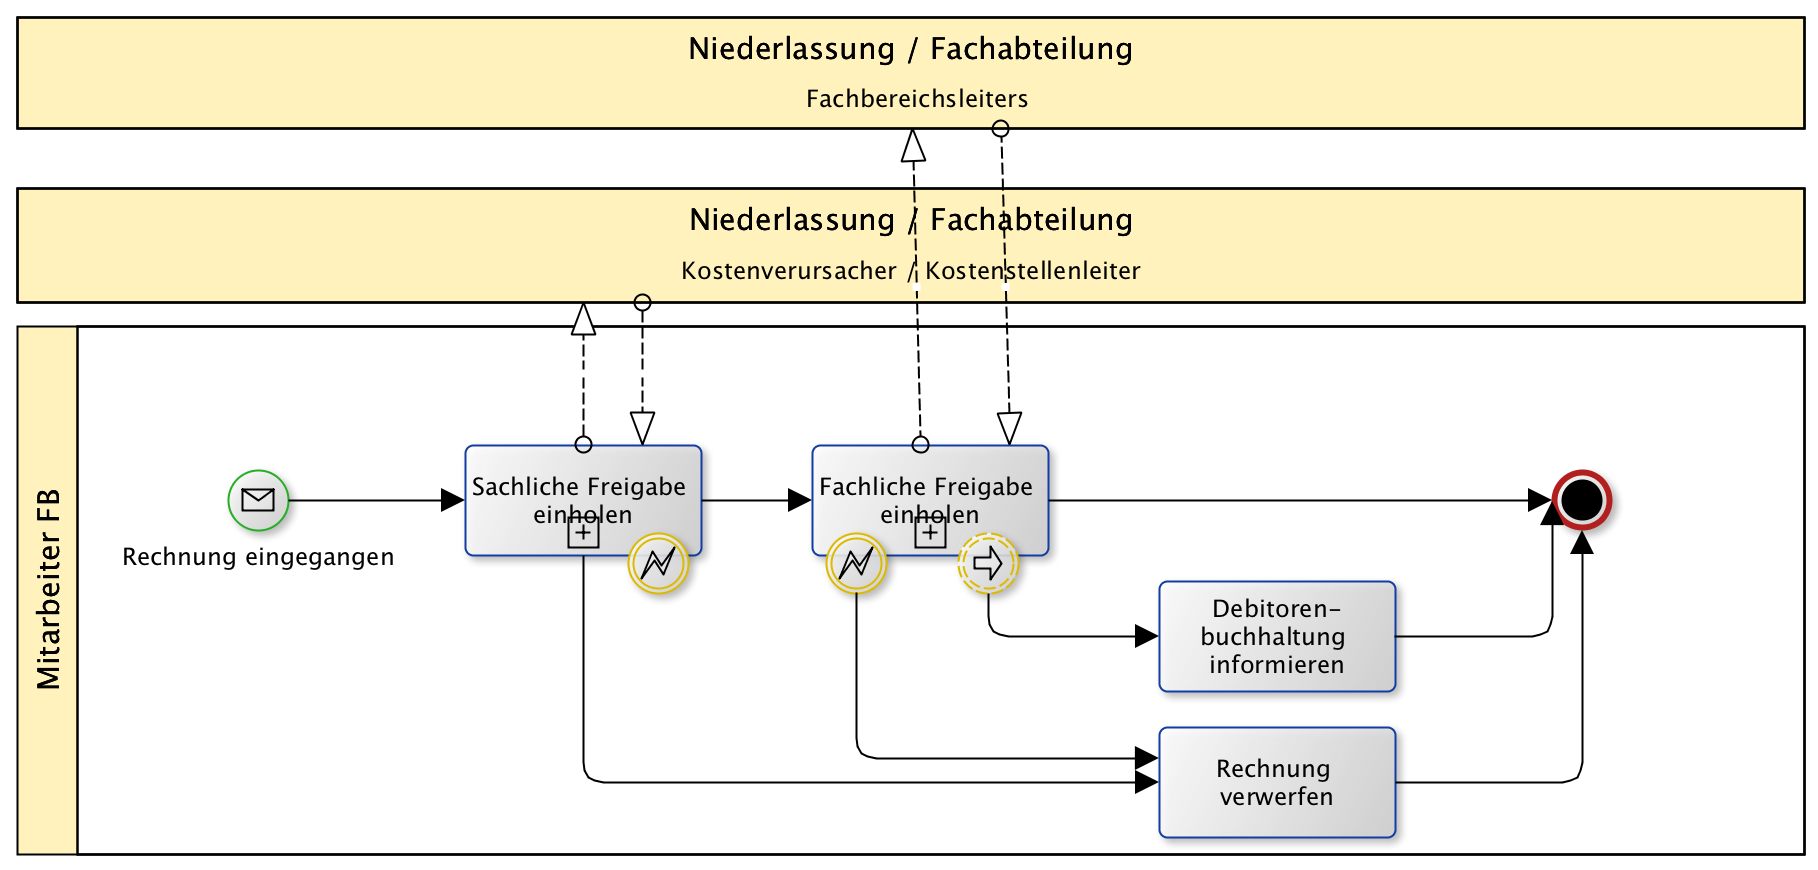
\includegraphics[height=75mm]{images/prozess_ist_simpel}
\caption{Der erste Teilprozess im Ist-Zustand}
\label{Teilprozess 1 im Ist-Zustand, BPMN simpel}
\end{figure}
\footnotetext{Quelle: Autor}

\subsection{Kreditorenworkflow Teil 2: Rechnungsbuchung}
Im zweiten Teil werden zur Buchung bereits Bestands-EDV-Systeme benutzt.
\subsubsection{Prozessablauf}
Zur Buchung werden alle eingescannten Versionen inklusive des Originals verwendet.
Zur Buchung wird der Beleg an Datev Rechnungswesen Pro übergeben.
Das Feature der automatischen Zeichenerkennung erkennt dabei insbesondere die Rechnungsnummer, das Datum, den Saldo und die Steuer.
Die Kostenstelle, sowie der Kostenträger müssen durch den Mitarbeiter angegeben werden.
In Datev wird die Rechnung dem Kreditor und unter diesem wiederum der Rechnungsnummer zugeordnet.
Damit ist die Rechnung in Datev verbucht.\\
Die Rechnung muss anschließend noch gezahlt werden.\\
Dazu wird ein Zahllauf in Datev angelegt.
In diesem erscheinen die fälligen Belege. 
Die Fälligkeit ergibt sich hierbei aus Rechnungsdatum und Zahlungsziel, welches aus den Kreditorenstammdaten entnommen wird.
Die fälligen Zahlungen werden nun zunächst durch den Mitarbeiter selbst geprüft.
Anschließend wird der Zahllauf dem Vorstandsvorsitzenden in Schriftform zur Freigabe vorgelegt.
Ist die Freigabe erfolgt, werden die in einer Datei an das eBanking-System gegeben.
Ein zweiter Mitarbeiter prüft die Freigabe durch den Vorstandsvorsitzenden und gibt die Zahlungen im eBanking-System frei.
Das eBanking-System übermittelt daraufhin die Zahlungen an die Bank, wo die Zahlung durchgeführt wird.
\subsubsection{Prozessmodellierung}

Auch dieser Teilprozess lässt sich mit dem gegebenen Ablauf modellieren. 
Die Durchführung der Zahlung kann als transparent betrachtet werden, da sie vollautomatisch durchgeführt wird.


\begin{figure}[!htb]
\centering
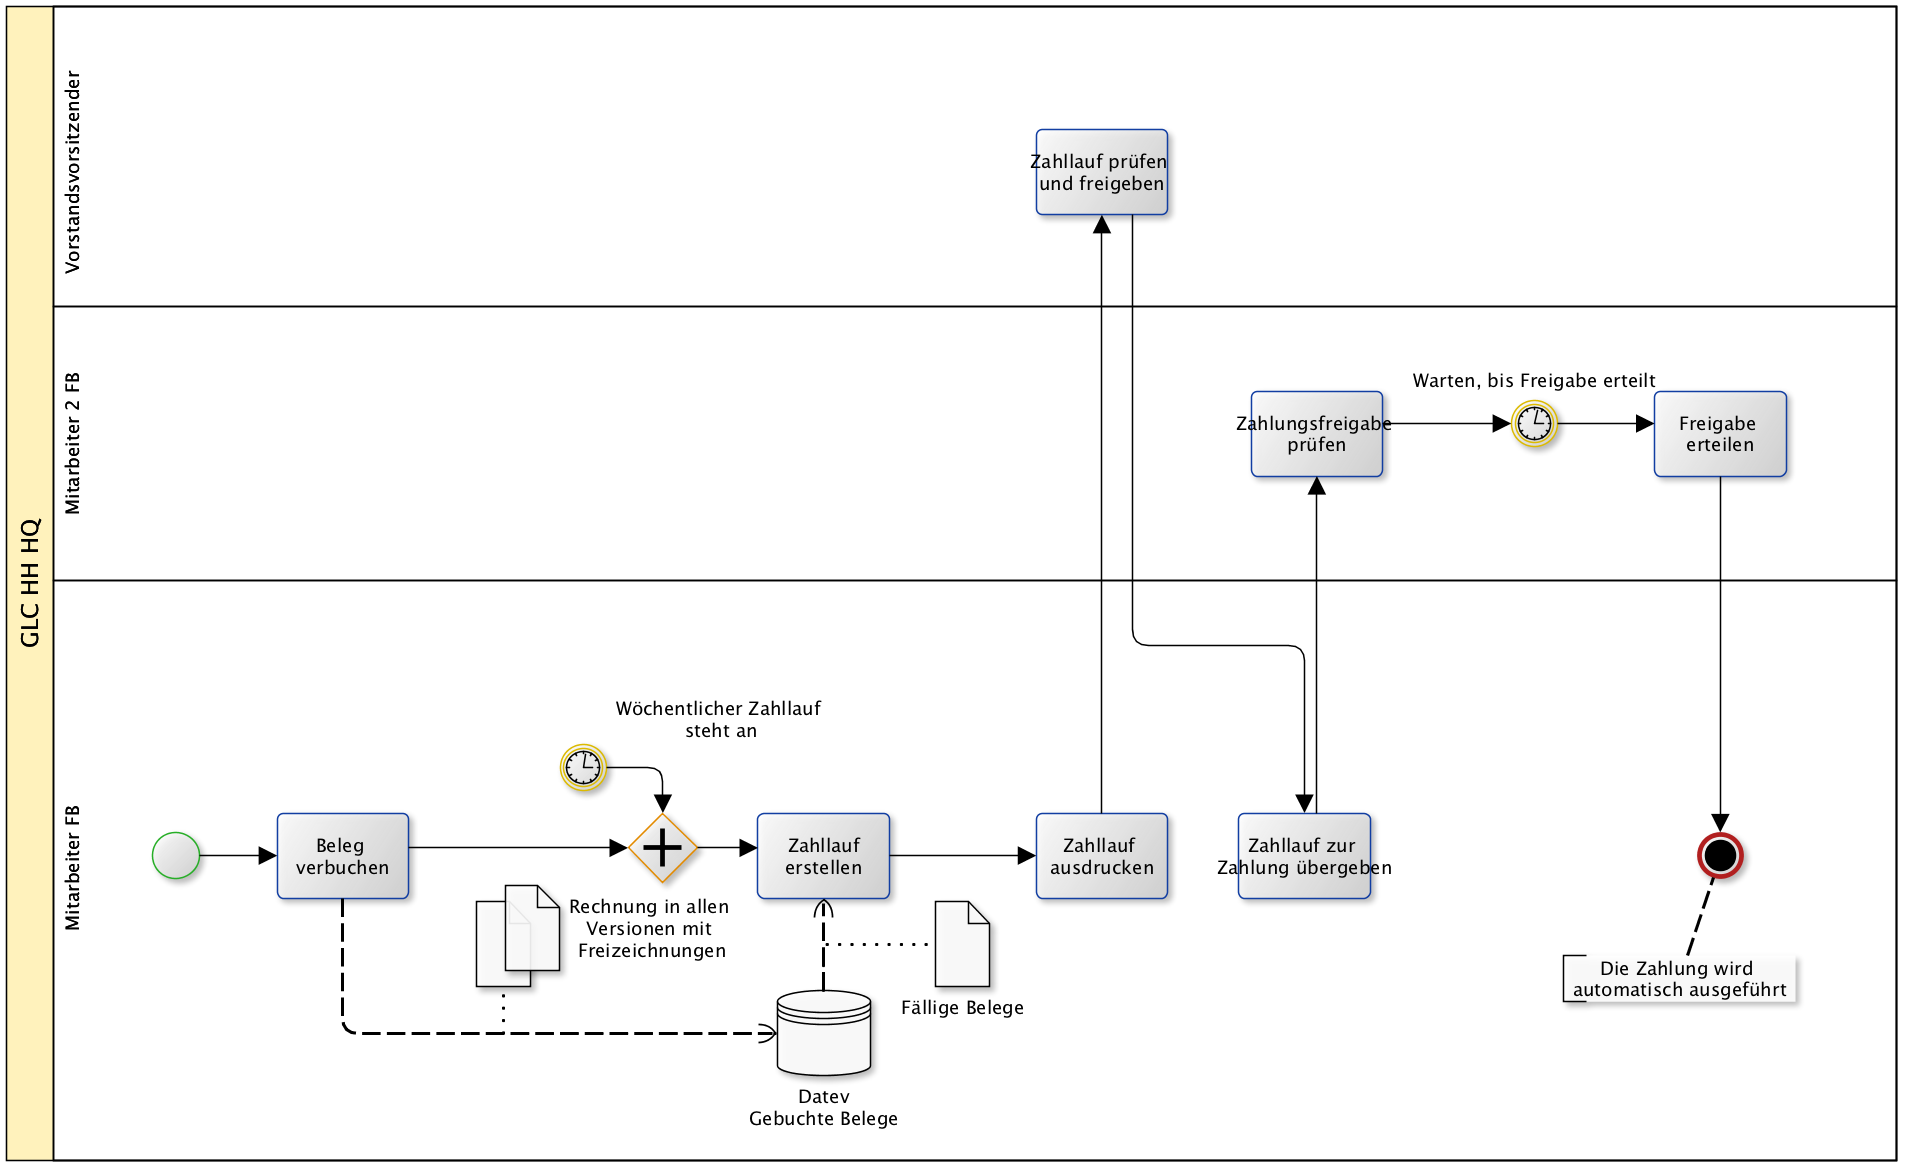
\includegraphics[height=90mm]{images/prozess_ist_buchung}
\caption{Der zweite Teilprozess im Ist-Zustand}
\label{Teilprozess 2 im Ist-Zustand, BPMN}
\end{figure}
\footnotetext{Quelle: Autor}
\newpage


\section{Problemanalyse}
Die nun folgende Problemanalyse ist Ausgangspunkt für die Neukonzeption.

\subsection{Methodik der Problemanalyse}
Zur Identifikation von problematischen Aspekten wird zunächst die argumentative Grundlage geschaffen, diese zweifelsfrei ermitteln zu können.
 dienen einerseits die Prozessbeschreibungen bzw. Prozessmodelle und andererseits die Interviews, die 
\subsubsection{Stakeholderanalyse}
Die Stakeholder des Prozesses ergeben sich aus den Akteuren, die in der Prozessbeschreibung bzw. der Prozessmodellierung als Beteiligte auftreten.\\
Das sind:


\begin{enumerate}
\item{Mitarbeiter der Finanzbuchhaltung}
\\ Speziell der Mitarbeiter der Finanzbuchhaltung, der für die Kreditorenbuchhaltung zuständig ist, ist in diesem Rahmen aktiv. 
\\ Ein weiterer Akteur aus diesem Bereich ist der (faktisch wechselnde) Mitarbeiter, der den Zahllauf nach dem Vieraugen-Prinzip freigibt. 
Dieser ist jedoch nur marginal beteiligt.
\\ Ein Stakholder, der nicht maßgeblich in diesem Prozess agiert, ist der Leiter der Finanzbuchhaltung, der die Prozesse der Abteilung plant, deren Implementation steuert und den Ablauf kontrolliert.

\item{Kostenstellenverantwortliche}
\\ Die Kostenverursacher sind Mitarbeiter, die zur Kostenverursachung befugt sind. 
Faktisch sind dies Kostenstellenverantwortliche, die regelmäßige oder abwicklungsbezogene Kosten verursachen und damit Kreditorenrechnungen auslösen. 
Durch sie erfolgt die sachliche Freigabe.

\item{EDV-Abteilung}
\\ Da der Prozess teilweise technologiegestützt abläuft, ist die Abteilung der Informationstechnologie, wenn auch nicht aktiv an Prozessinstanzen beteiligt, als Stakeholder auszumachen. 

\item{Bereichsverantwortliche}
\\ Die Mitarbeiter, die die fachliche Freigabe erteilen dürfen, sind Bereichsleiter. 
Konkret lässt sich dies zum Zeitpunkt der Erstellung dieser Arbeit auf drei Personen konkretisieren. 
Von diesen befinden sich zwei im Vorstand, der dritte ist der Bereichsleiter Informationstechnologie.\\

\end{enumerate}

Aus dieser Liste lassen sich konkrete Personen ableiten, deren Erfahrung mit dem Prozess zur Problemidentifikation dienen kann. 
Mit diesen werden Interviews geführt, um eine empirische Grundlage zu schaffen.

Es ergeben sich:

\begin{enumerate}
\item{Mitarbeiter der (Kreditoren-)Buchhaltung}
\item{Leiter der Finanzbuchhaltung}
\item{Ein Bereichsverantwortlicher}
\item{Leiter der Informationstechnologie}
\end{enumerate}


\subsubsection{Beschreibung und Modellierung der Teilprozesse}

Auch die erarbeiteten Abläufe der Teilprozesse dienen als Grundlage der Analyse.


\subsection{Fehler}
Eine von zwei Möglichkeiten, die im Zusammenhang mit dem Prozess problematisch sind, sind fehlerhafte Prozessinstanzen. Als fehlerhaft wird eine Prozessinstanz betrachtet, wenn diese nicht wie beschrieben abläuft, also der Modellierung nicht folgt.
\subsubsection{Fehlerarten}

\begin{enumerate}
\item{Rechnung nicht zugegen}
\\ Die Rechnung befindet sich zu einem bestimmten Zeitpunkt nicht am vorgesehenen Ort. 
Sie ist entweder nicht in die Finanzbuchhaltung gegeben worden oder auf sonstige Art auf dem Weg des Freigabeprozesses verloren gegangen.
\item{Formal nicht korrekte Rechnung}
\\ Die Rechnung weist nicht alle Daten auf, die zur sachlichen und fachlichen Freigabe ggf. nötig wären, sodass Rücksprache mit dem Kreditor notwendig ist.
\end{enumerate}


\subsubsection{Fehlerquellen}

Die Fehlerquellen sind aus den Interviews ersichtlich. 
Die bereitgestellten Systeme werden als adäquat und funktional betrachtet.
Als problematisch wird nur der Teil empfunden, in dem keine IT-System-seitige Prozessunterstützung stattfindet.
Die Gründe für fehlerhafte Prozessinstanzen sind demnach auf menschliches Verhalten zurückzuführen, welches in diesem Zusammenhang durch Nachlässigkeit die beschrieben Fehler auslöst.
\\
Bezüglich fehlerhafter Rechnungen ist die Ursache meistens auf Nachlässigkeit seitens des Kreditors zurückzuführen.
Da diese von internen Prozessen losgelöst ist, steht diese Fehlerquelle nicht im Fokus dieser Arbeit. 

\subsection{Performance}
Die zweite Möglichkeit für eine als problematisch wahrgenommene Prozessinstanz ist deren mangelhafte Performance.
Diesbezüglich gibt es mehrere Anhaltspunkte, die von Stakeholdern angesprochen werden.
Zum einen gestalten sich Prozessdurchläufe langwierig.
Unabhängig davon, ob die Freizeichnung mit Akteuren durchgeführt wird, die sich inner- oder außerhalb der Unternehmenszentrale befinden und dementsprechend eine räumliche Entfernung zwischen der Finanzbuchhaltung und den Freizeichnern ergibt vorliegt oder nicht, ist der Freigabeprozess mit hohem manuellen Kommunikationsaufwand verbunden, der über E-Mail oder direkt, allerdings mit Laufwegen durch das Unternehmen bearbeitet wird.
\\
Aus diesem Umstand ergibt sich auch die mangelhafte Kontrollmöglichkeit, sowohl für den betroffenen Mitarbeiter der Finanzbuchhaltung, sowie die mit der Freizeichnung beauftragten Akteure, da sich Rechnungen in der zu einem bestimmten Zeitpunkt aktuellen Version faktisch nur im Zugriff eines einzelnen Mitarbeiters befinden. 
Besonders deutlich wird diese Situation bei Rechnungen, die innerhalb der Unternehmenszentrale durchgereicht werden.
An jeder Station (also Rechnungsannahme, sachliche Freigabe, fachliche Freigabe und wieder zurück in der Finanzbuchhaltung) besteht zusätzlich die Möglichkeit, dass ein Beleg abhanden kommt und eine neue Prozessinstanz erst durch Nachsendung einer Mahnung oder Zahlungserinnerung ausgelöst wird.

\subsubsection{Key Performance Indicators}
Diese Kritikpunkte lassen sich in objektiven Kennzahlen ausdrücken, an denen der Prozess im Ist-Zustand gemessen werden kann. 
Diese sollen auch die Neukonzeption des Prozesses begleiten, bzw. diese an der Verbesserung resultierender Werte ausgerichtet werden.
Auf Basis der Erläuterungen in 3.2 und in diesem Kapitel ergeben sich zwei Kennzahlen:

\begin{enumerate}
\item{Prozesslaufzeit}
\\ Die objektiv messbare Zeit von Rechnungseingang/-annahme bis Bezahlung, speziell jedoch in dem als performanceschwach wahrgenommenen Teil von Rechnungseingang/-annahme bis Buchung.
\item{Prozessfehlerrate}
\\ Relativer Anteil fehlerhafter Prozessinstanzen.
\end{enumerate}



